\documentclass[./main.tex]{subfiles}

\begin{document}
\section{Experiment}\label{experiement}
Throughout the following section the results and configuration details of our trained model are described and explained. In the first section, Section \ref{subsec:conf_details}, the configuration details of the model, as well as the training of the model, are described. In the second section, Section \ref{subsec:results}, the results of training the Stacked hourglass is presented, as well as a short discussion of which version of the model which will be used going forward. In the last section, Section \ref{subsec:training_details}, we give an overview of the technical details behind training the network, which can be followed in case the reader has any technical problems in case of testing for reproducibility.

\subsection{Configuration Details}\label{subsec:conf_details}
Our model only consists of a single hourglass. The hourglass consists of $4$ down- and upsamples. The module uses a single residual between each down- and upsample, as well as $3$ residuals in the bottleneck. Newell \textit{et al.} \cite{Newell} and Olsen \cite{Camilla} experiment with different amount of hourglasses and with different amount of residual modules in each hourglass. They conclude, that stacking multiple hourglasses or using hourglasses with multiple residual modules between each down- and upsample increases the performance of the model. However, as the main purpose of this section is not to create a model with state-of-the-art results, but instead to create a model that can be interpreted and explored, we have chosen to reduce the size of the model. For the same reasons, we will not be developing and testing various configurations of the architecture. Likewise, the purpose of this section is neither to improve the model developed by Newell \textit{et. al} \cite{Newell}, hence why we will be making the same configuration choices as Newell \textit{et. al} \cite{Newell} and Olsen \cite{Camilla}, which are described in the following.
\\
\\
To prevent the model from overfitting we use batch normalization. Newell \textit{et al.} does not describe where to perform the batch normalization, so we follow Olsen \cite{Camilla} and perform the batch normalization before each convolutional layer in each residual module, after the first convolutional layer of the entire network and before the last convolutional layer of the entire network. For the choice of acitvation function we use ReLU after each batch normalization. Each max pooling and nearest neighbor upsampling uses a kernel size and stride of $2$, which halves and doubles the size of the input, respectively. The full network has been visualized in Figure \ref{fig:architecture}.
\\
\begin{figure}[p]
    \centering
    \begin{subfigure}{5 cm}
        \centering
        
\includegraphics[width =  5 cm]{entities/residual_drawing.png}
        \caption{The Residual module}
    \end{subfigure}
    \begin{subfigure}{5 cm}
        \centering
        
\includegraphics[width = 5 cm]{entities/hourglass_drawing.png}
        \caption{The Hourglass}
    \end{subfigure}
    \begin{subfigure}{5 cm}
        \centering
        
\includegraphics[width = 4 cm]{entities/SHG_drawing.png}
        \caption{The Full network}
    \end{subfigure}
    \caption{Overview of the used architecture}
    \label{fig:architecture}
\end{figure}
\\
For the initial values of the weights we initialize each weight by sampling from a \textit{Glorot normal distribution} (also known as a \textit{Xavier normal distribution}), described as
$$\mathcal{N} \left(0, \frac{2}{fan_{in} + fan_{out}} \right)$$
where $fan_{in}$ is the amount of input connections and $fan_{out}$ is the amount of output connections to the layer of the weight \cite{Xavier}. By doing so we make all layers have the same activation variance and gradient variance, essentially helping the model to converge \cite{DeepLearning}.
\\
\\
We make use of a mini-batch size of $16$ and no data augmentation, since the dataset is already rather large and captures a lot of the variances. To optimize the network we make use of $MSE$ as our loss function, \textit{RMSProp} with momentum paramter $\alpha = 0.99$ as our optimizer, as well as use a initial learning rate of $2.5e-4$ as done by Newell \textit{et al.} \cite{Newell} and Olsen \cite{Camilla}. We decided to use a mini-batch size of $16$ as Olsen experienced great results with this mini-batch size \cite{Camilla}, as well as it being the biggest mini-batch size that our machine could run.
\\
\\
After each epoch we find the validation accuracy of the model by computing the PCK between the predictions and the ground truth of the validation dataset.  For the two constants for $PCK$, $c$ (the normalization constant) and $r$ (the threshold radius), we follow Olsen \cite{Camilla} by letting $c$ be one tenth of the heatmap resolution size $\left(\text{that is, }\frac{64}{10} = 6.4 \right)$ and $r$ be $0.5$.
\\
\\
While training the model the PCK accuracy is computed after each epoch, keeping track of the best PCK accuracy. The first time the best PCK accuracy has not improved for $5$ continuous epochs, the learning rate is dropped by a factor of $5$ permanently, helping the training loss reach a minimum.
\\
\\
We do not make use of automated stopping criterias, such as \textit{automated early stopping}, as these have certain parameters that can be difficult to choose. Instead, we train the network and save a copy of the model after each epoch. While the training is happening, we note the training loss, validation loss as well as the validation PCK accuracy of the model after each epoch, and stop the training process in case the model does not improve for a while.

\subsection{Results}\label{subsec:results}
\begin{figure}[htbp]
    \centering
    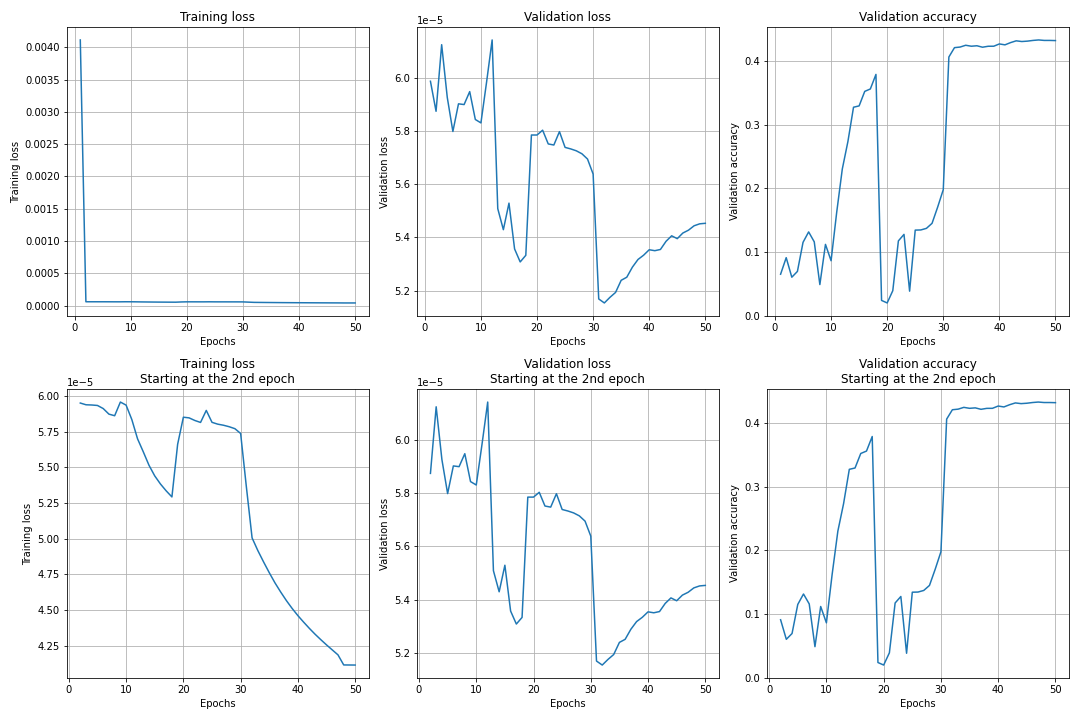
\includegraphics[width = \textwidth]{entities/results.png}
    \caption{Visualization of the evolution of the training loss, validation loss and validation PCK accuracy of the trained model. Top row shows all of the $50$ epochs. Bottom row shows epoch $2$ and forward to ease the reading of the training loss}
    \label{fig:results}
\end{figure}
\noindent In Figure \ref{fig:results}, the evolution of the training loss, validation loss and validation PCK accuracy is visualized. The model were initially set to train for $100$ epochs, however, we decided to stop the training early, as the PCK validation accuracy seemed to have converged, as well as the model clearly started to overfit after $32$ epochs, as seen by comparing the training and validation loss.
\\
\\
The reduction of the learning rate happened after $21$ epochs. By looking at the validation accuracy in Figure \ref{fig:results} we can see, that the accuracy rapidly increases shortly after the reduction of the learning rate, hinting at the effectiveness of dropping the learning rate. 
\\
\\
Comparing the training loss, validation loss and the validation accuracy we see, that the there is not an overlap between the models yielding the best training loss, validation loss and validation accuracy. As we in section \ref{sec:XAI} want to explore a model that performs decently well, we will be using the model with the highest validation accuracy as our model going forward. Thus, our model is the model from epoch $47$, which has a training loss of $4.19 \cdot 10^{-5}$, a validation loss of $5.43 \cdot 10^{-5}$ and a validation accuracy of $0.433$. If we test the model on the held-out testing set from Section \ref{sec:dataset}, we get a PCK score of $0.441$, which is based on all annotated keypoints (that is, both for $v = 1$ and $v = 2$)

\subsection{Training Details}\label{subsec:training_details}
The Stacked hourglass was implemented in Python 3.8.2 using PyTorch version 1.7.1 and Cuda version 10.2 on a machine using Windows 10 version 20H2, build 19042. The network was trained on an 8 GB NVIDIA GeForce GTX 1070 GPU using a Samsung 840 EVO SSD for data storage. Training the network takes about $70$ minutes per epoch, totalling to about $58$ hours for $50$ epochs.

\end{document}